\begin{frame}[title-small={color=hpiorange, bg=none, text=Context}]
	\maketitle
\end{frame}


\begin{frame}{Notations}
  \begin{minipage}{1.0\textwidth}
    \begin{itemize}
      \item state vector: $|\psi\rangle$, arbitrary quantum state $\psi$
      \item state vector: $|0\rangle$, $|1\rangle$, classical states $0$ and $1$ respectively
      \item density matrix: $\rho = \Sigma_{i=1}^{n} p_i |\psi_i\rangle \langle\psi_i |$, probabilities $p_i$, $\Sigma_{i} p_i = 1$, dimensions $n$
      \begin{itemize}
        \item example\footnote{[Melke2010]}: two qubits entangled state $\frac{1}{\sqrt{2}} ( |00\rangle + |11\rangle ) = \frac{1}{\sqrt{2}} (1, 0, 0, 1)^T $
        \item example density matrix: $\rho = \frac{1}{\sqrt{2}} (1, 0, 0, 1)^T \frac{1}{\sqrt{2}} (1, 0, 0, 1) = \begin{bmatrix} 1 & 0 & 0 & 1 \\ 0 & 0 & 0 & 0 \\ 0 & 0 & 0 & 0 \\ 1 & 0 & 0 & 1\end{bmatrix}$
      \end{itemize}
      \item covariance matrix: $\Sigma$
      \begin{itemize}
        \item example\footnote{[Lokho2020]}: two feature sets $X$ and $Y$
        \item example covariance matrix: $\Sigma = \begin{bmatrix} E(X \otimes X) & E(X \otimes Y) \\ E(Y \otimes X) & E(Y \otimes Y)\end{bmatrix}$, with $E(A)$ the expectation value of $A$
      \end{itemize}
    \end{itemize}
  \end{minipage}
\end{frame}


\begin{frame}{Classical PCA}
  \begin{minipage}{0.5\textwidth}
    \centering
    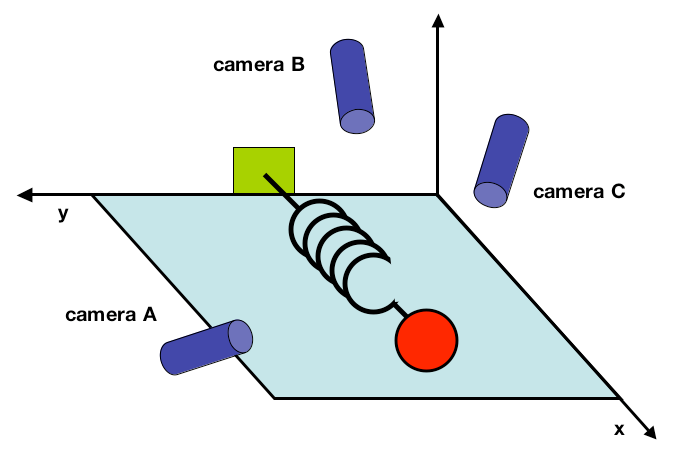
\includegraphics[width=\textwidth]{../assets/context_pca_example.png}
  \end{minipage}%
  \begin{minipage}{0.5\textwidth}
    \begin{itemize}
      \item problem: high dimensional data $\rightarrow$ which features are relevant?
      \item idea: reduce total amount of features
      \item techniques: eigenvalue decomposition, singular value tresholding
    \end{itemize}
  \end{minipage}
  \footnote{[Shlen2014]}
\end{frame}


\begin{frame}{Quantum PCA}
  \begin{minipage}{1.0\textwidth}
    \centering
    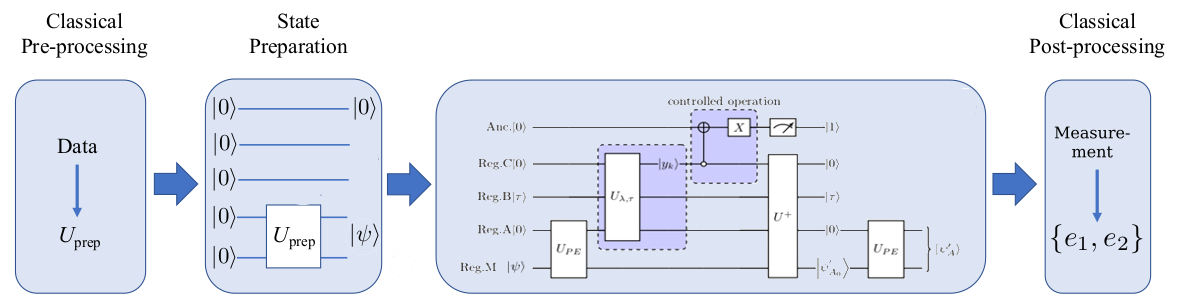
\includegraphics[width=\textwidth]{../assets/context_algorithm_main-2.png}
  \end{minipage}
  \hfill
  \footnote{[Lokho2020], [He2021]}
  \begin{minipage}{1.0\textwidth}
    \begin{itemize}
      \item operation $U_{PE}$: quantum phase estimation
      \item operation $U_{\lambda, r}$: singular value tresholding
    \end{itemize}
  \end{minipage}
\end{frame}


\begin{frame}{Quantum PCA}
  \begin{minipage}{1.0\textwidth}
    \centering
    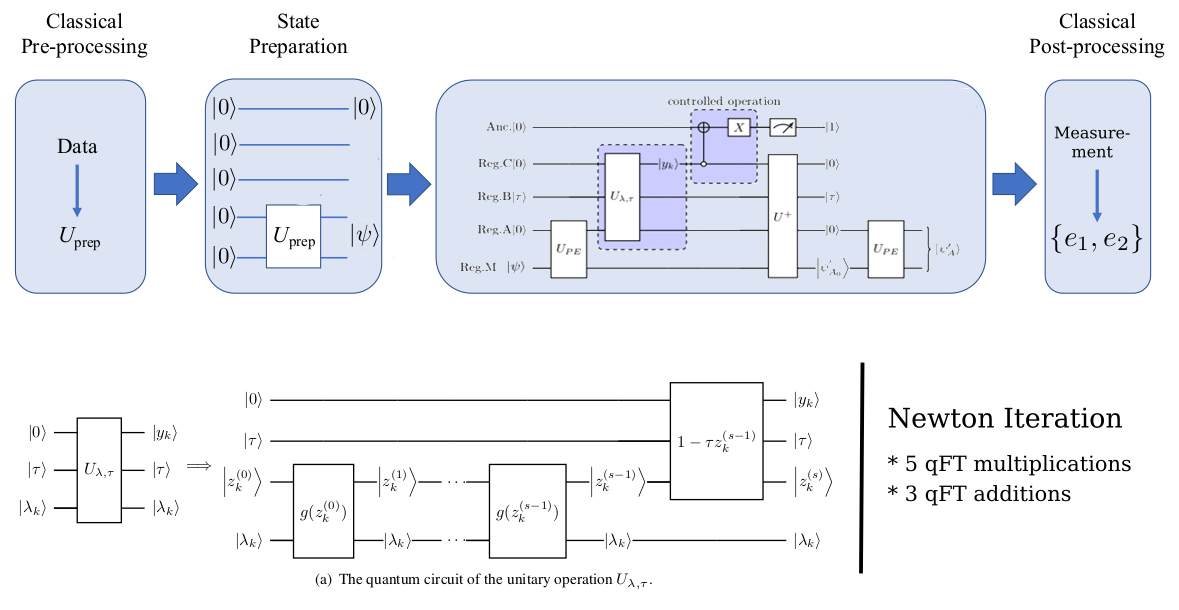
\includegraphics[width=\textwidth]{../assets/context_algorithm_main-3.png}
  \end{minipage}
  \footnote{[Lokho2020], [He2021]}
\end{frame}


\begin{frame}{Quantum PCA}
  \begin{minipage}{1.0\textwidth}
    \centering
    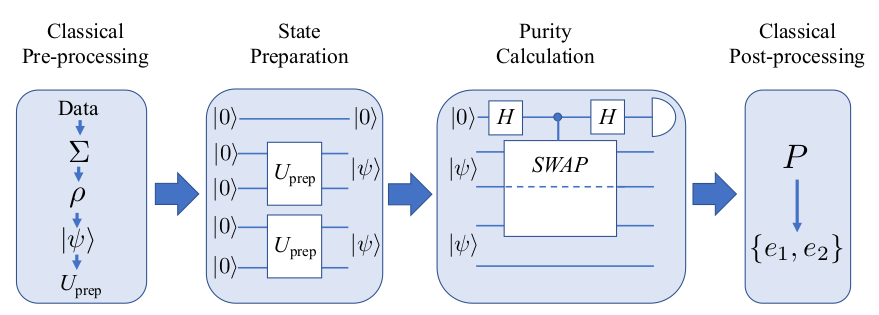
\includegraphics[width=\textwidth]{../assets/context_algorithm_main-ref19.png}
  \end{minipage}
  \footnote{[Lokho2020]}
  \hfill
  \begin{minipage}{1.0\textwidth}
    \begin{itemize}
      \item change 1: no singular value tresholding $\rightarrow$ post processing
      \item change 2: swap test instead of quantum phase estimation
      \item limitation: only $2 \times 2$ matrices $\Sigma$
    \end{itemize}
  \end{minipage}
\end{frame}
